%% discarded-exception.tex
%%
%% "It Is Not the Cryptography: A Discarded Exception Dominates Token
%%  Validation Cost in a Node.js Service"
%%
%% Clean rewrite from the evidence. Supersedes key-resolution-cost.tex, which
%% was patched through two reframings; that file is retained as a fallback.
%%
%% EVERY numeric value is a macro from keypath_macros.tex, generated by
%% analysis/make_keypath_macros.py from files under data/runs/ and survey/.
%% No digit is typed in the body. keypath_macros_provenance.csv maps each macro
%% to the file it was read from.
\documentclass[pdflatex,sn-basic]{sn-jnl}

\usepackage{lmodern}
\usepackage{manyfoot}
\usepackage{amsmath}
\usepackage{amssymb}
\usepackage{graphicx}
\usepackage{booktabs}
\usepackage{url}
\usepackage{xcolor}

% keypath_macros.tex -- GENERATED. Do not edit.
% Regenerate: .venv/bin/python -m analysis.make_keypath_macros
% Every value below is read from a file under data/runs/ or survey/.
\providecommand{\PLACEHOLDER}[1]{\textcolor{red}{\textbf{[MISSING: #1]}}}

\newcommand{\AbCpuDelta}{76.92}% data/runs/INSITU-AB-authmode-jwt/openloop_ramp.csv
\newcommand{\AbCpuJwt}{146.38}% data/runs/INSITU-AB-authmode-jwt/openloop_ramp.csv
\newcommand{\AbCpuNone}{69.45}% data/runs/INSITU-AB-authmode-none/openloop_ramp.csv
\newcommand{\AbCpuPerCallDelta}{384.6}% data/runs/INSITU-AB-authmode-jwt/openloop_ramp.csv
\newcommand{\AbCpuPerCallJwt}{731.9}% data/runs/INSITU-AB-authmode-jwt/openloop_ramp.csv
\newcommand{\AbCpuPerCallNone}{347.3}% data/runs/INSITU-AB-authmode-none/openloop_ramp.csv
\newcommand{\AbCpuSampleMaxJwt}{183.299}% data/runs/INSITU-AB-authmode-jwt/pod_cpu_samples.csv
\newcommand{\AbCpuSampleMaxNone}{100.577}% data/runs/INSITU-AB-authmode-none/pod_cpu_samples.csv
\newcommand{\AbCpuSampleMinJwt}{114.963}% data/runs/INSITU-AB-authmode-jwt/pod_cpu_samples.csv
\newcommand{\AbCpuSampleMinNone}{53.088}% data/runs/INSITU-AB-authmode-none/pod_cpu_samples.csv
\newcommand{\AbCpuSamplesJwt}{127}% data/runs/INSITU-AB-authmode-jwt/pod_cpu_samples.csv
\newcommand{\AbCpuSamplesNone}{127}% data/runs/INSITU-AB-authmode-none/pod_cpu_samples.csv
\newcommand{\AbEventLoopLagJwt}{3.159}% data/runs/INSITU-AB-authmode-jwt/openloop_ramp.csv
\newcommand{\AbEventLoopLagNone}{3.137}% data/runs/INSITU-AB-authmode-none/openloop_ramp.csv
\newcommand{\AbGapSeconds}{78}% data/runs/INSITU-AB-authmode-jwt/run_metadata.json
\newcommand{\AbLatencyDeltaUs}{353.0}% data/runs/INSITU-AB-authmode-jwt/openloop_ramp.csv
\newcommand{\AbLatencyJwt}{2.0332}% data/runs/INSITU-AB-authmode-jwt/openloop_ramp.csv
\newcommand{\AbLatencyNone}{1.6802}% data/runs/INSITU-AB-authmode-none/openloop_ramp.csv
\newcommand{\AbLatencyPNineNineJwt}{8.0890}% data/runs/INSITU-AB-authmode-jwt/openloop_ramp.csv
\newcommand{\AbLatencyPNineNineNone}{6.3480}% data/runs/INSITU-AB-authmode-none/openloop_ramp.csv
\newcommand{\AbLoadFifteenJwt}{3.49}% data/runs/INSITU-AB-authmode-jwt/run_metadata.json
\newcommand{\AbLoadFifteenNone}{3.18}% data/runs/INSITU-AB-authmode-none/run_metadata.json
\newcommand{\AbLoadFiveJwt}{4.10}% data/runs/INSITU-AB-authmode-jwt/run_metadata.json
\newcommand{\AbLoadFiveNone}{3.50}% data/runs/INSITU-AB-authmode-none/run_metadata.json
\newcommand{\AbLoadOneJwt}{5.11}% data/runs/INSITU-AB-authmode-jwt/run_metadata.json
\newcommand{\AbLoadOneNone}{3.53}% data/runs/INSITU-AB-authmode-none/run_metadata.json
\newcommand{\AbRateJwt}{200.006}% data/runs/INSITU-AB-authmode-jwt/openloop_ramp.csv
\newcommand{\AbRateNone}{200.006}% data/runs/INSITU-AB-authmode-none/openloop_ramp.csv
\newcommand{\AbRequestsJwt}{36001}% data/runs/INSITU-AB-authmode-jwt/k6_summary.json
\newcommand{\AbRequestsNone}{36001}% data/runs/INSITU-AB-authmode-none/k6_summary.json
\newcommand{\AbSidecarCpuJwt}{49.13}% data/runs/INSITU-AB-authmode-jwt/openloop_ramp.csv
\newcommand{\AbSidecarCpuNone}{53.40}% data/runs/INSITU-AB-authmode-none/openloop_ramp.csv
\newcommand{\AbTopProcPctJwt}{84.3}% data/runs/INSITU-AB-authmode-jwt/run_metadata.json
\newcommand{\AbTopProcPctNone}{135.1}% data/runs/INSITU-AB-authmode-none/run_metadata.json
\newcommand{\AbWindowSecondsJwt}{180}% data/runs/INSITU-AB-authmode-jwt/k6_summary.json
\newcommand{\AbWindowSecondsNone}{180}% data/runs/INSITU-AB-authmode-none/k6_summary.json
\newcommand{\AdjudicatedFalsePositive}{5}% survey/data/hand_adjudication.csv
\newcommand{\AdjudicatedGenuine}{7}% survey/data/hand_adjudication.csv
\newcommand{\AdjudicatedGenuinePct}{5.36}% survey/data/hand_adjudication.csv
\newcommand{\AdjudicatedGenuineProjects}{6}% survey/data/hand_adjudication.csv
\newcommand{\AdjudicatedTotal}{13}% survey/data/hand_adjudication.csv
\newcommand{\AdjudicatedUnresolved}{1}% survey/data/hand_adjudication.csv
\newcommand{\ContainerVersusHostRatio}{0.92}% data/runs/2026-09-17T08-57-13Z-keypath-runtime-matrix/keypath_stats.json
\newcommand{\CounterFilesFetched}{191}% survey/data/counterexamples.json
\newcommand{\CounterReposWithVerify}{112}% survey/data/counterexamples.json
\newcommand{\CounterWithVerify}{120}% survey/data/counterexamples.json
\newcommand{\DecompExplainedPct}{77.9}% data/runs/2026-09-17T08-42-17Z-keypath-mechanism/keypath_stats.json
\newcommand{\DecompObserved}{23.92}% data/runs/2026-09-17T08-42-17Z-keypath-mechanism/keypath_stats.json
\newcommand{\DecompPredicted}{18.62}% data/runs/2026-09-17T08-42-17Z-keypath-mechanism/keypath_stats.json
\newcommand{\DecompResidual}{5.292}% data/runs/2026-09-17T08-42-17Z-keypath-mechanism/keypath_stats.json
\newcommand{\DecompResidualCiHi}{5.501}% data/runs/2026-09-17T08-42-17Z-keypath-mechanism/keypath_stats.json
\newcommand{\DecompResidualCiLo}{4.916}% data/runs/2026-09-17T08-42-17Z-keypath-mechanism/keypath_stats.json
\newcommand{\HostCallsPerInvocation}{40000}% data/runs/2026-09-17T08-42-17Z-keypath-mechanism/keypath_stats.json
\newcommand{\HostCreateSecretKey}{0.583}% data/runs/2026-09-17T08-42-17Z-keypath-mechanism/keypath_stats.json
\newcommand{\HostCreateSecretKeyCiHi}{0.583}% data/runs/2026-09-17T08-42-17Z-keypath-mechanism/keypath_stats.json
\newcommand{\HostCreateSecretKeyCiLo}{0.542}% data/runs/2026-09-17T08-42-17Z-keypath-mechanism/keypath_stats.json
\newcommand{\HostCvMax}{3.5}% data/runs/2026-09-17T08-42-17Z-keypath-mechanism/keypath_stats.json
\newcommand{\HostDecodeOnly}{1.292}% data/runs/2026-09-17T08-42-17Z-keypath-mechanism/keypath_stats.json
\newcommand{\HostDecodeOnlyCiHi}{1.292}% data/runs/2026-09-17T08-42-17Z-keypath-mechanism/keypath_stats.json
\newcommand{\HostDecodeOnlyCiLo}{1.250}% data/runs/2026-09-17T08-42-17Z-keypath-mechanism/keypath_stats.json
\newcommand{\HostHmacKeyObject}{2.166}% data/runs/2026-09-17T08-42-17Z-keypath-mechanism/keypath_stats.json
\newcommand{\HostHmacKeyObjectCiHi}{2.167}% data/runs/2026-09-17T08-42-17Z-keypath-mechanism/keypath_stats.json
\newcommand{\HostHmacKeyObjectCiLo}{2.125}% data/runs/2026-09-17T08-42-17Z-keypath-mechanism/keypath_stats.json
\newcommand{\HostHmacString}{2.208}% data/runs/2026-09-17T08-42-17Z-keypath-mechanism/keypath_stats.json
\newcommand{\HostHmacStringCiHi}{2.250}% data/runs/2026-09-17T08-42-17Z-keypath-mechanism/keypath_stats.json
\newcommand{\HostHmacStringCiLo}{2.208}% data/runs/2026-09-17T08-42-17Z-keypath-mechanism/keypath_stats.json
\newcommand{\HostInvocations}{15}% data/runs/2026-09-17T08-42-17Z-keypath-mechanism/keypath_stats.json
\newcommand{\HostJwtPreparsed}{6.042}% data/runs/2026-09-17T08-42-17Z-keypath-mechanism/keypath_stats.json
\newcommand{\HostJwtPreparsedCiHi}{6.125}% data/runs/2026-09-17T08-42-17Z-keypath-mechanism/keypath_stats.json
\newcommand{\HostJwtPreparsedCiLo}{5.958}% data/runs/2026-09-17T08-42-17Z-keypath-mechanism/keypath_stats.json
\newcommand{\HostJwtRsPemString}{52.58}% data/runs/2026-09-17T08-42-17Z-keypath-mechanism/keypath_stats.json
\newcommand{\HostJwtRsPemStringCiHi}{52.71}% data/runs/2026-09-17T08-42-17Z-keypath-mechanism/keypath_stats.json
\newcommand{\HostJwtRsPemStringCiLo}{52.42}% data/runs/2026-09-17T08-42-17Z-keypath-mechanism/keypath_stats.json
\newcommand{\HostJwtRsPreparsed}{25.33}% data/runs/2026-09-17T08-42-17Z-keypath-mechanism/keypath_stats.json
\newcommand{\HostJwtRsPreparsedCiHi}{25.50}% data/runs/2026-09-17T08-42-17Z-keypath-mechanism/keypath_stats.json
\newcommand{\HostJwtRsPreparsedCiLo}{25.29}% data/runs/2026-09-17T08-42-17Z-keypath-mechanism/keypath_stats.json
\newcommand{\HostJwtString}{29.92}% data/runs/2026-09-17T08-42-17Z-keypath-mechanism/keypath_stats.json
\newcommand{\HostJwtStringCiHi}{30.12}% data/runs/2026-09-17T08-42-17Z-keypath-mechanism/keypath_stats.json
\newcommand{\HostJwtStringCiLo}{29.75}% data/runs/2026-09-17T08-42-17Z-keypath-mechanism/keypath_stats.json
\newcommand{\HostJwtStringSafe}{7.208}% data/runs/2026-09-17T08-42-17Z-keypath-mechanism/keypath_stats.json
\newcommand{\HostJwtStringSafeCiHi}{7.334}% data/runs/2026-09-17T08-42-17Z-keypath-mechanism/keypath_stats.json
\newcommand{\HostJwtStringSafeCiLo}{7.125}% data/runs/2026-09-17T08-42-17Z-keypath-mechanism/keypath_stats.json
\newcommand{\HostNodeVersion}{26.6.0}% data/runs/2026-09-17T08-42-17Z-keypath-mechanism/keypath_stats.json
\newcommand{\HostProbeShareOfCall}{60}% data/runs/2026-09-17T08-42-17Z-keypath-mechanism/keypath_stats.json
\newcommand{\HostProbeSucceeds}{13.83}% data/runs/2026-09-17T08-42-17Z-keypath-mechanism/keypath_stats.json
\newcommand{\HostProbeSucceedsCiHi}{13.92}% data/runs/2026-09-17T08-42-17Z-keypath-mechanism/keypath_stats.json
\newcommand{\HostProbeSucceedsCiLo}{13.62}% data/runs/2026-09-17T08-42-17Z-keypath-mechanism/keypath_stats.json
\newcommand{\HostProbeThrows}{18.04}% data/runs/2026-09-17T08-42-17Z-keypath-mechanism/keypath_stats.json
\newcommand{\HostProbeThrowsCiHi}{18.25}% data/runs/2026-09-17T08-42-17Z-keypath-mechanism/keypath_stats.json
\newcommand{\HostProbeThrowsCiLo}{17.83}% data/runs/2026-09-17T08-42-17Z-keypath-mechanism/keypath_stats.json
\newcommand{\HostRsStringPenalty}{27.29}% data/runs/2026-09-17T08-42-17Z-keypath-mechanism/keypath_stats.json
\newcommand{\HostRsStringPenaltyCiHi}{27.37}% data/runs/2026-09-17T08-42-17Z-keypath-mechanism/keypath_stats.json
\newcommand{\HostRsStringPenaltyCiLo}{27.00}% data/runs/2026-09-17T08-42-17Z-keypath-mechanism/keypath_stats.json
\newcommand{\HostRsStringPenaltyRounds}{15}% data/runs/2026-09-17T08-42-17Z-keypath-mechanism/keypath_stats.json
\newcommand{\HostSafePatchRatio}{4.15}% data/runs/2026-09-17T08-42-17Z-keypath-mechanism/keypath_stats.json
\newcommand{\HostSafePatchResidual}{1.208}% data/runs/2026-09-17T08-42-17Z-keypath-mechanism/keypath_stats.json
\newcommand{\HostSafePatchResidualCiHi}{1.251}% data/runs/2026-09-17T08-42-17Z-keypath-mechanism/keypath_stats.json
\newcommand{\HostSafePatchResidualCiLo}{1.084}% data/runs/2026-09-17T08-42-17Z-keypath-mechanism/keypath_stats.json
\newcommand{\HostSafePatchResidualRounds}{15}% data/runs/2026-09-17T08-42-17Z-keypath-mechanism/keypath_stats.json
\newcommand{\HostSafePatchSaving}{22.71}% data/runs/2026-09-17T08-42-17Z-keypath-mechanism/keypath_stats.json
\newcommand{\HostSafePatchSavingCiHi}{22.88}% data/runs/2026-09-17T08-42-17Z-keypath-mechanism/keypath_stats.json
\newcommand{\HostSafePatchSavingCiLo}{22.54}% data/runs/2026-09-17T08-42-17Z-keypath-mechanism/keypath_stats.json
\newcommand{\HostSafePatchSavingRounds}{15}% data/runs/2026-09-17T08-42-17Z-keypath-mechanism/keypath_stats.json
\newcommand{\HostStringPenalty}{23.92}% data/runs/2026-09-17T08-42-17Z-keypath-mechanism/keypath_stats.json
\newcommand{\HostStringPenaltyCiHi}{24.00}% data/runs/2026-09-17T08-42-17Z-keypath-mechanism/keypath_stats.json
\newcommand{\HostStringPenaltyCiLo}{23.58}% data/runs/2026-09-17T08-42-17Z-keypath-mechanism/keypath_stats.json
\newcommand{\HostStringPenaltyRounds}{15}% data/runs/2026-09-17T08-42-17Z-keypath-mechanism/keypath_stats.json
\newcommand{\HostTimerOverhead}{0.042}% data/runs/2026-09-17T08-42-17Z-keypath-mechanism/keypath_stats.json
\newcommand{\HostTimerOverheadCiHi}{0.042}% data/runs/2026-09-17T08-42-17Z-keypath-mechanism/keypath_stats.json
\newcommand{\HostTimerOverheadCiLo}{0.042}% data/runs/2026-09-17T08-42-17Z-keypath-mechanism/keypath_stats.json
\newcommand{\HostVeight}{14}% data/runs/2026-09-17T08-42-17Z-keypath-mechanism/run_metadata.json
\newcommand{\HostVeightFull}{14.6.202.34-node.26}% data/runs/2026-09-17T08-42-17Z-keypath-mechanism/run_metadata.json
\newcommand{\IdentityMismatches}{0}% data/runs/2026-09-17T08-57-13Z-keypath-runtime-matrix/environments.csv
\newcommand{\InsituObservedHi}{1028}% data/runs/2026-09-14T05-57-22Z-verifyrate-hs256/verify_rate_curve.csv
\newcommand{\InsituObservedLo}{453}% data/runs/2026-09-14T05-57-22Z-verifyrate-hs256/verify_rate_curve.csv
\newcommand{\InsituPredictedFromMatrix}{381}% data/runs/2026-09-17T08-57-13Z-keypath-runtime-matrix/keypath_stats.json
\newcommand{\InsituPreparsedAscA}{221.42}% data/runs/2026-09-14T15-01-36Z-verifyrate-hs256-preparsed/verify_rate_curve.csv
\newcommand{\InsituPreparsedAscB}{235.01}% data/runs/2026-09-14T15-01-36Z-verifyrate-hs256-preparsed/verify_rate_curve.csv
\newcommand{\InsituPreparsedAscC}{168.44}% data/runs/2026-09-14T15-01-36Z-verifyrate-hs256-preparsed/verify_rate_curve.csv
\newcommand{\InsituPreparsedAscD}{127.19}% data/runs/2026-09-14T15-01-36Z-verifyrate-hs256-preparsed/verify_rate_curve.csv
\newcommand{\InsituPreparsedAscE}{79.70}% data/runs/2026-09-14T15-01-36Z-verifyrate-hs256-preparsed/verify_rate_curve.csv
\newcommand{\InsituPreparsedAscF}{71.68}% data/runs/2026-09-14T15-01-36Z-verifyrate-hs256-preparsed/verify_rate_curve.csv
\newcommand{\InsituPreparsedAscG}{39.38}% data/runs/2026-09-14T15-01-36Z-verifyrate-hs256-preparsed/verify_rate_curve.csv
\newcommand{\InsituPreparsedDescA}{200.88}% data/runs/2026-09-14T15-01-36Z-verifyrate-hs256-preparsed/verify_rate_curve.csv
\newcommand{\InsituPreparsedDescB}{188.06}% data/runs/2026-09-14T15-01-36Z-verifyrate-hs256-preparsed/verify_rate_curve.csv
\newcommand{\InsituPreparsedDescC}{160.58}% data/runs/2026-09-14T15-01-36Z-verifyrate-hs256-preparsed/verify_rate_curve.csv
\newcommand{\InsituPreparsedDescD}{116.67}% data/runs/2026-09-14T15-01-36Z-verifyrate-hs256-preparsed/verify_rate_curve.csv
\newcommand{\InsituPreparsedDescE}{66.93}% data/runs/2026-09-14T15-01-36Z-verifyrate-hs256-preparsed/verify_rate_curve.csv
\newcommand{\InsituPreparsedDescF}{42.78}% data/runs/2026-09-14T15-01-36Z-verifyrate-hs256-preparsed/verify_rate_curve.csv
\newcommand{\InsituPreparsedDescG}{34.61}% data/runs/2026-09-14T15-01-36Z-verifyrate-hs256-preparsed/verify_rate_curve.csv
\newcommand{\InsituPreparsedPoints}{7}% data/runs/2026-09-14T15-01-36Z-verifyrate-hs256-preparsed/verify_rate_curve.csv
\newcommand{\InsituPreparsedSameSign}{7}% data/runs/2026-09-14T15-01-36Z-verifyrate-hs256-preparsed/verify_rate_curve.csv
\newcommand{\InsituRateA}{5}% data/runs/2026-09-14T05-57-22Z-verifyrate-hs256/verify_rate_curve.csv
\newcommand{\InsituRateB}{10}% data/runs/2026-09-14T05-57-22Z-verifyrate-hs256/verify_rate_curve.csv
\newcommand{\InsituRateC}{25}% data/runs/2026-09-14T05-57-22Z-verifyrate-hs256/verify_rate_curve.csv
\newcommand{\InsituRateD}{50}% data/runs/2026-09-14T05-57-22Z-verifyrate-hs256/verify_rate_curve.csv
\newcommand{\InsituRateE}{100}% data/runs/2026-09-14T05-57-22Z-verifyrate-hs256/verify_rate_curve.csv
\newcommand{\InsituRateF}{200}% data/runs/2026-09-14T05-57-22Z-verifyrate-hs256/verify_rate_curve.csv
\newcommand{\InsituRateG}{400}% data/runs/2026-09-14T05-57-22Z-verifyrate-hs256/verify_rate_curve.csv
\newcommand{\InsituRsAscA}{351.05}% data/runs/2026-09-14T06-41-56Z-verifyrate-rs256/verify_rate_curve.csv
\newcommand{\InsituRsAscB}{338.89}% data/runs/2026-09-14T06-41-56Z-verifyrate-rs256/verify_rate_curve.csv
\newcommand{\InsituRsAscC}{270.77}% data/runs/2026-09-14T06-41-56Z-verifyrate-rs256/verify_rate_curve.csv
\newcommand{\InsituRsAscD}{203.19}% data/runs/2026-09-14T06-41-56Z-verifyrate-rs256/verify_rate_curve.csv
\newcommand{\InsituRsAscE}{120.42}% data/runs/2026-09-14T06-41-56Z-verifyrate-rs256/verify_rate_curve.csv
\newcommand{\InsituRsAscF}{73.92}% data/runs/2026-09-14T06-41-56Z-verifyrate-rs256/verify_rate_curve.csv
\newcommand{\InsituRsAscG}{59.11}% data/runs/2026-09-14T06-41-56Z-verifyrate-rs256/verify_rate_curve.csv
\newcommand{\InsituRsDescA}{292.11}% data/runs/2026-09-14T06-41-56Z-verifyrate-rs256/verify_rate_curve.csv
\newcommand{\InsituRsDescB}{286.13}% data/runs/2026-09-14T06-41-56Z-verifyrate-rs256/verify_rate_curve.csv
\newcommand{\InsituRsDescC}{251.70}% data/runs/2026-09-14T06-41-56Z-verifyrate-rs256/verify_rate_curve.csv
\newcommand{\InsituRsDescD}{193.82}% data/runs/2026-09-14T06-41-56Z-verifyrate-rs256/verify_rate_curve.csv
\newcommand{\InsituRsDescE}{111.88}% data/runs/2026-09-14T06-41-56Z-verifyrate-rs256/verify_rate_curve.csv
\newcommand{\InsituRsDescF}{73.94}% data/runs/2026-09-14T06-41-56Z-verifyrate-rs256/verify_rate_curve.csv
\newcommand{\InsituRsDescG}{58.88}% data/runs/2026-09-14T06-41-56Z-verifyrate-rs256/verify_rate_curve.csv
\newcommand{\InsituRsPoints}{7}% data/runs/2026-09-14T06-41-56Z-verifyrate-rs256/verify_rate_curve.csv
\newcommand{\InsituRsSameSign}{6}% data/runs/2026-09-14T06-41-56Z-verifyrate-rs256/verify_rate_curve.csv
\newcommand{\InsituStringAscA}{928.24}% data/runs/2026-09-14T05-57-22Z-verifyrate-hs256/verify_rate_curve.csv
\newcommand{\InsituStringAscB}{976.28}% data/runs/2026-09-14T05-57-22Z-verifyrate-hs256/verify_rate_curve.csv
\newcommand{\InsituStringAscC}{918.54}% data/runs/2026-09-14T05-57-22Z-verifyrate-hs256/verify_rate_curve.csv
\newcommand{\InsituStringAscD}{758.57}% data/runs/2026-09-14T05-57-22Z-verifyrate-hs256/verify_rate_curve.csv
\newcommand{\InsituStringAscE}{571.59}% data/runs/2026-09-14T05-57-22Z-verifyrate-hs256/verify_rate_curve.csv
\newcommand{\InsituStringAscF}{494.91}% data/runs/2026-09-14T05-57-22Z-verifyrate-hs256/verify_rate_curve.csv
\newcommand{\InsituStringAscG}{452.82}% data/runs/2026-09-14T05-57-22Z-verifyrate-hs256/verify_rate_curve.csv
\newcommand{\InsituStringDescA}{1027.97}% data/runs/2026-09-14T05-57-22Z-verifyrate-hs256/verify_rate_curve.csv
\newcommand{\InsituStringDescB}{1017.34}% data/runs/2026-09-14T05-57-22Z-verifyrate-hs256/verify_rate_curve.csv
\newcommand{\InsituStringDescC}{934.47}% data/runs/2026-09-14T05-57-22Z-verifyrate-hs256/verify_rate_curve.csv
\newcommand{\InsituStringDescD}{737.12}% data/runs/2026-09-14T05-57-22Z-verifyrate-hs256/verify_rate_curve.csv
\newcommand{\InsituStringDescE}{607.78}% data/runs/2026-09-14T05-57-22Z-verifyrate-hs256/verify_rate_curve.csv
\newcommand{\InsituStringDescF}{532.50}% data/runs/2026-09-14T05-57-22Z-verifyrate-hs256/verify_rate_curve.csv
\newcommand{\InsituStringDescG}{467.62}% data/runs/2026-09-14T05-57-22Z-verifyrate-hs256/verify_rate_curve.csv
\newcommand{\InsituStringPoints}{7}% data/runs/2026-09-14T05-57-22Z-verifyrate-hs256/verify_rate_curve.csv
\newcommand{\InsituStringSameSign}{6}% data/runs/2026-09-14T05-57-22Z-verifyrate-hs256/verify_rate_curve.csv
\newcommand{\InsituTightestAgreement}{0.02}% data/runs/2026-09-14T06-41-56Z-verifyrate-rs256/verify_rate_curve.csv
\newcommand{\InsituUnaccountedHi}{647}% data/runs/2026-09-14T05-57-22Z-verifyrate-hs256/verify_rate_curve.csv
\newcommand{\InsituUnaccountedLo}{71}% data/runs/2026-09-14T05-57-22Z-verifyrate-hs256/verify_rate_curve.csv
\newcommand{\ManifestFiles}{502}% survey/data/corpus_manifest.csv
\newcommand{\ManifestHeadResolved}{501}% survey/data/corpus_manifest.csv
\newcommand{\ManifestRepos}{457}% survey/data/corpus_manifest.csv
\newcommand{\ManifestSampleFiles}{311}% survey/data/corpus_manifest.csv
\newcommand{\MatrixCallsPerInvocation}{20000}% data/runs/2026-09-17T08-57-13Z-keypath-runtime-matrix/keypath_stats.json
\newcommand{\MatrixCvMax}{20.2}% data/runs/2026-09-17T08-57-13Z-keypath-runtime-matrix/keypath_stats.json
\newcommand{\MatrixCvMaxCondition}{probe\_succeeds}% data/runs/2026-09-17T08-57-13Z-keypath-runtime-matrix/keypath_stats.json
\newcommand{\MatrixCvMaxEnvironment}{node:26.6.0-bookworm}% data/runs/2026-09-17T08-57-13Z-keypath-runtime-matrix/keypath_stats.json
\newcommand{\MatrixCvRatio}{5.7}% data/runs/2026-09-17T08-57-13Z-keypath-runtime-matrix/keypath_stats.json
\newcommand{\MatrixInvocations}{10}% data/runs/2026-09-17T08-57-13Z-keypath-runtime-matrix/keypath_stats.json
\newcommand{\NodeEighteenDecodeOnly}{1.62}% data/runs/2026-09-17T08-57-13Z-keypath-runtime-matrix/keypath_stats.json
\newcommand{\NodeEighteenHmacString}{2.42}% data/runs/2026-09-17T08-57-13Z-keypath-runtime-matrix/keypath_stats.json
\newcommand{\NodeEighteenImageId}{8d6421d663b4}% data/runs/runtime_identity.csv
\newcommand{\NodeEighteenJwtPreparsed}{7.58}% data/runs/2026-09-17T08-57-13Z-keypath-runtime-matrix/keypath_stats.json
\newcommand{\NodeEighteenJwtString}{394.71}% data/runs/2026-09-17T08-57-13Z-keypath-runtime-matrix/keypath_stats.json
\newcommand{\NodeEighteenNodeLiteral}{18.20.8}% data/runs/2026-09-17T08-57-13Z-keypath-runtime-matrix/keypath_stats.json
\newcommand{\NodeEighteenNodeMajor}{18}% data/runs/2026-09-17T08-57-13Z-keypath-runtime-matrix/keypath_stats.json
\newcommand{\NodeEighteenOpensslLiteral}{3.0.16}% data/runs/2026-09-17T08-57-13Z-keypath-runtime-matrix/keypath_stats.json
\newcommand{\NodeEighteenOpensslSeries}{3.0}% data/runs/2026-09-17T08-57-13Z-keypath-runtime-matrix/keypath_stats.json
\newcommand{\NodeEighteenProbeSucceeds}{115.83}% data/runs/2026-09-17T08-57-13Z-keypath-runtime-matrix/keypath_stats.json
\newcommand{\NodeEighteenProbeThrows}{373.79}% data/runs/2026-09-17T08-57-13Z-keypath-runtime-matrix/keypath_stats.json
\newcommand{\NodeEighteenProbeThrowsCiHi}{375.79}% data/runs/2026-09-17T08-57-13Z-keypath-runtime-matrix/keypath_stats.json
\newcommand{\NodeEighteenProbeThrowsCiLo}{371.50}% data/runs/2026-09-17T08-57-13Z-keypath-runtime-matrix/keypath_stats.json
\newcommand{\NodeEighteenVeight}{10}% data/runs/runtime_identity.csv
\newcommand{\NodeEighteenVeightFull}{10.2.154.26-node.39}% data/runs/runtime_identity.csv
\newcommand{\NodeTwentyDecodeOnly}{2.19}% data/runs/2026-09-17T08-57-13Z-keypath-runtime-matrix/keypath_stats.json
\newcommand{\NodeTwentyHmacString}{2.33}% data/runs/2026-09-17T08-57-13Z-keypath-runtime-matrix/keypath_stats.json
\newcommand{\NodeTwentyImageId}{fb4cd12c85ee}% data/runs/runtime_identity.csv
\newcommand{\NodeTwentyJwtPreparsed}{7.25}% data/runs/2026-09-17T08-57-13Z-keypath-runtime-matrix/keypath_stats.json
\newcommand{\NodeTwentyJwtString}{437.40}% data/runs/2026-09-17T08-57-13Z-keypath-runtime-matrix/keypath_stats.json
\newcommand{\NodeTwentyNodeLiteral}{20.20.2}% data/runs/2026-09-17T08-57-13Z-keypath-runtime-matrix/keypath_stats.json
\newcommand{\NodeTwentyNodeMajor}{20}% data/runs/2026-09-17T08-57-13Z-keypath-runtime-matrix/keypath_stats.json
\newcommand{\NodeTwentyOpensslLiteral}{3.0.19}% data/runs/2026-09-17T08-57-13Z-keypath-runtime-matrix/keypath_stats.json
\newcommand{\NodeTwentyOpensslSeries}{3.0}% data/runs/2026-09-17T08-57-13Z-keypath-runtime-matrix/keypath_stats.json
\newcommand{\NodeTwentyProbeSucceeds}{142.38}% data/runs/2026-09-17T08-57-13Z-keypath-runtime-matrix/keypath_stats.json
\newcommand{\NodeTwentyProbeThrows}{420.62}% data/runs/2026-09-17T08-57-13Z-keypath-runtime-matrix/keypath_stats.json
\newcommand{\NodeTwentyProbeThrowsCiHi}{422.56}% data/runs/2026-09-17T08-57-13Z-keypath-runtime-matrix/keypath_stats.json
\newcommand{\NodeTwentyProbeThrowsCiLo}{419.52}% data/runs/2026-09-17T08-57-13Z-keypath-runtime-matrix/keypath_stats.json
\newcommand{\NodeTwentySixGlibcDecodeOnly}{1.67}% data/runs/2026-09-17T08-57-13Z-keypath-runtime-matrix/keypath_stats.json
\newcommand{\NodeTwentySixGlibcHmacString}{3.19}% data/runs/2026-09-17T08-57-13Z-keypath-runtime-matrix/keypath_stats.json
\newcommand{\NodeTwentySixGlibcImageId}{6e0a69f43d2b}% data/runs/runtime_identity.csv
\newcommand{\NodeTwentySixGlibcJwtPreparsed}{6.04}% data/runs/2026-09-17T08-57-13Z-keypath-runtime-matrix/keypath_stats.json
\newcommand{\NodeTwentySixGlibcJwtString}{27.96}% data/runs/2026-09-17T08-57-13Z-keypath-runtime-matrix/keypath_stats.json
\newcommand{\NodeTwentySixGlibcNodeLiteral}{26.6.0}% data/runs/2026-09-17T08-57-13Z-keypath-runtime-matrix/keypath_stats.json
\newcommand{\NodeTwentySixGlibcNodeMajor}{26}% data/runs/2026-09-17T08-57-13Z-keypath-runtime-matrix/keypath_stats.json
\newcommand{\NodeTwentySixGlibcOpensslLiteral}{3.5.7}% data/runs/2026-09-17T08-57-13Z-keypath-runtime-matrix/keypath_stats.json
\newcommand{\NodeTwentySixGlibcOpensslSeries}{3.5}% data/runs/2026-09-17T08-57-13Z-keypath-runtime-matrix/keypath_stats.json
\newcommand{\NodeTwentySixGlibcProbeSucceeds}{12.12}% data/runs/2026-09-17T08-57-13Z-keypath-runtime-matrix/keypath_stats.json
\newcommand{\NodeTwentySixGlibcProbeThrows}{16.58}% data/runs/2026-09-17T08-57-13Z-keypath-runtime-matrix/keypath_stats.json
\newcommand{\NodeTwentySixGlibcProbeThrowsCiHi}{17.88}% data/runs/2026-09-17T08-57-13Z-keypath-runtime-matrix/keypath_stats.json
\newcommand{\NodeTwentySixGlibcProbeThrowsCiLo}{16.38}% data/runs/2026-09-17T08-57-13Z-keypath-runtime-matrix/keypath_stats.json
\newcommand{\NodeTwentySixGlibcVeight}{14}% data/runs/runtime_identity.csv
\newcommand{\NodeTwentySixGlibcVeightFull}{14.6.202.34-node.26}% data/runs/runtime_identity.csv
\newcommand{\NodeTwentySixMuslDecodeOnly}{1.71}% data/runs/2026-09-17T08-57-13Z-keypath-runtime-matrix/keypath_stats.json
\newcommand{\NodeTwentySixMuslHmacString}{3.25}% data/runs/2026-09-17T08-57-13Z-keypath-runtime-matrix/keypath_stats.json
\newcommand{\NodeTwentySixMuslImageId}{a4fb14143ee2}% data/runs/runtime_identity.csv
\newcommand{\NodeTwentySixMuslJwtPreparsed}{6.56}% data/runs/2026-09-17T08-57-13Z-keypath-runtime-matrix/keypath_stats.json
\newcommand{\NodeTwentySixMuslJwtString}{36.42}% data/runs/2026-09-17T08-57-13Z-keypath-runtime-matrix/keypath_stats.json
\newcommand{\NodeTwentySixMuslNodeLiteral}{26.6.0}% data/runs/2026-09-17T08-57-13Z-keypath-runtime-matrix/keypath_stats.json
\newcommand{\NodeTwentySixMuslNodeMajor}{26}% data/runs/2026-09-17T08-57-13Z-keypath-runtime-matrix/keypath_stats.json
\newcommand{\NodeTwentySixMuslOpensslLiteral}{3.5.7}% data/runs/2026-09-17T08-57-13Z-keypath-runtime-matrix/keypath_stats.json
\newcommand{\NodeTwentySixMuslOpensslSeries}{3.5}% data/runs/2026-09-17T08-57-13Z-keypath-runtime-matrix/keypath_stats.json
\newcommand{\NodeTwentySixMuslProbeSucceeds}{15.54}% data/runs/2026-09-17T08-57-13Z-keypath-runtime-matrix/keypath_stats.json
\newcommand{\NodeTwentySixMuslProbeThrows}{22.94}% data/runs/2026-09-17T08-57-13Z-keypath-runtime-matrix/keypath_stats.json
\newcommand{\NodeTwentySixMuslProbeThrowsCiHi}{23.29}% data/runs/2026-09-17T08-57-13Z-keypath-runtime-matrix/keypath_stats.json
\newcommand{\NodeTwentySixMuslProbeThrowsCiLo}{22.79}% data/runs/2026-09-17T08-57-13Z-keypath-runtime-matrix/keypath_stats.json
\newcommand{\NodeTwentySixMuslVeight}{14}% data/runs/runtime_identity.csv
\newcommand{\NodeTwentySixMuslVeightFull}{14.6.202.34-node.26}% data/runs/runtime_identity.csv
\newcommand{\NodeTwentyVeight}{11}% data/runs/runtime_identity.csv
\newcommand{\NodeTwentyVeightFull}{11.3.244.8-node.38}% data/runs/runtime_identity.csv
\newcommand{\PopBestCellPct}{0.0000}% survey/data/population_counts.csv
\newcommand{\PopCapturedAt}{2026-09-18}% survey/data/population_counts.csv
\newcommand{\PopJsImportFiles}{524288}% survey/data/population_counts.csv
\newcommand{\PopJsImportFilesWithApi}{38}% survey/data/population_counts.csv
\newcommand{\PopJsImportPct}{0.0072}% survey/data/population_counts.csv
\newcommand{\PopJsRequireFiles}{790528}% survey/data/population_counts.csv
\newcommand{\PopJsRequireFilesWithApi}{29}% survey/data/population_counts.csv
\newcommand{\PopJsRequirePct}{0.0037}% survey/data/population_counts.csv
\newcommand{\PopLargestCellFiles}{790528}% survey/data/population_counts.csv
\newcommand{\PopSumFiles}{1656928}% survey/data/population_counts.csv
\newcommand{\PopSumFilesWithApi}{168}% survey/data/population_counts.csv
\newcommand{\PopSumOneIn}{9863}% survey/data/population_counts.csv
\newcommand{\PopSumPct}{0.0101}% survey/data/population_counts.csv
\newcommand{\PopTsImportFiles}{333824}% survey/data/population_counts.csv
\newcommand{\PopTsImportFilesWithApi}{101}% survey/data/population_counts.csv
\newcommand{\PopTsImportPct}{0.0303}% survey/data/population_counts.csv
\newcommand{\PopTsRequireFiles}{8288}% survey/data/population_counts.csv
\newcommand{\PopTsRequireFilesWithApi}{0}% survey/data/population_counts.csv
\newcommand{\PopTsRequirePct}{0.0000}% survey/data/population_counts.csv
\newcommand{\PopWorstCellPct}{0.0303}% survey/data/population_counts.csv
\newcommand{\PreparsedUnattributed}{2.58}% data/runs/2026-09-17T08-42-17Z-keypath-mechanism/keypath_stats.json
\newcommand{\ProfEighteenPct}{95.3}% data/runs/2026-09-18T-profile-matched/cpuprof_matched.csv
\newcommand{\ProfEighteenPctHi}{95.6}% data/runs/2026-09-18T-profile-matched/cpuprof_matched.csv
\newcommand{\ProfEighteenPctLo}{95.1}% data/runs/2026-09-18T-profile-matched/cpuprof_matched.csv
\newcommand{\ProfHostPct}{66.2}% data/runs/2026-09-18T-profile-matched/cpuprof_matched.csv
\newcommand{\ProfHostPctHi}{67.4}% data/runs/2026-09-18T-profile-matched/cpuprof_matched.csv
\newcommand{\ProfHostPctLo}{65.3}% data/runs/2026-09-18T-profile-matched/cpuprof_matched.csv
\newcommand{\ProfIterations}{50000}% data/runs/2026-09-18T-profile-matched/cpuprof_matched.csv
\newcommand{\ProfRepeats}{3}% data/runs/2026-09-18T-profile-matched/cpuprof_matched.csv
\newcommand{\ProfTwentySixPct}{61.5}% data/runs/2026-09-18T-profile-matched/cpuprof_matched.csv
\newcommand{\ProfTwentySixPctHi}{61.6}% data/runs/2026-09-18T-profile-matched/cpuprof_matched.csv
\newcommand{\ProfTwentySixPctLo}{58.5}% data/runs/2026-09-18T-profile-matched/cpuprof_matched.csv
\newcommand{\RematchAdjudicated}{12}% survey/data/hand_adjudication.csv
\newcommand{\RematchSitesPreparsed}{0}% survey/data/hand_adjudication.csv
\newcommand{\SampleBuffer}{2}% survey/data/callsites.csv
\newcommand{\SampleCallSites}{327}% survey/data/callsites.csv
\newcommand{\SampleEnvString}{176}% survey/data/callsites.csv
\newcommand{\SampleFileContents}{4}% survey/data/callsites.csv
\newcommand{\SampleNoAlgorithms}{309}% survey/data/callsites.csv
\newcommand{\SampleNoAlgorithmsPct}{94}% survey/data/callsites.csv
\newcommand{\SampleRematchAdded}{12}% survey/data/callsites.csv
\newcommand{\SampleRepos}{247}% survey/data/callsites.csv
\newcommand{\SampleSitesPreparsed}{0}% survey/data/callsites.csv
\newcommand{\SampleStringLiteral}{52}% survey/data/callsites.csv
\newcommand{\SampleUnknown}{93}% survey/data/callsites.csv
\newcommand{\SpanDecodeOnly}{1.35}% data/runs/2026-09-17T08-57-13Z-keypath-runtime-matrix/keypath_stats.json
\newcommand{\SpanDecodeOnlyWithHost}{1.69}% data/runs/2026-09-17T08-57-13Z-keypath-runtime-matrix/keypath_stats.json
\newcommand{\SpanHmacString}{1.39}% data/runs/2026-09-17T08-57-13Z-keypath-runtime-matrix/keypath_stats.json
\newcommand{\SpanHmacStringWithHost}{1.47}% data/runs/2026-09-17T08-57-13Z-keypath-runtime-matrix/keypath_stats.json
\newcommand{\SpanJwtPreparsed}{1.26}% data/runs/2026-09-17T08-57-13Z-keypath-runtime-matrix/keypath_stats.json
\newcommand{\SpanJwtPreparsedWithHost}{1.26}% data/runs/2026-09-17T08-57-13Z-keypath-runtime-matrix/keypath_stats.json
\newcommand{\SpanProbeSucceeds}{11.74}% data/runs/2026-09-17T08-57-13Z-keypath-runtime-matrix/keypath_stats.json
\newcommand{\SpanProbeSucceedsWithHost}{11.74}% data/runs/2026-09-17T08-57-13Z-keypath-runtime-matrix/keypath_stats.json
\newcommand{\SpanProbeThrows}{25.36}% data/runs/2026-09-17T08-57-13Z-keypath-runtime-matrix/keypath_stats.json
\newcommand{\SpanProbeThrowsWithHost}{25.36}% data/runs/2026-09-17T08-57-13Z-keypath-runtime-matrix/keypath_stats.json
\newcommand{\SuiteNaiveFailing}{2}% data/runs/2026-09-18T-upstream-suite/suite_results.csv
\newcommand{\SuiteNaivePassing}{509}% data/runs/2026-09-18T-upstream-suite/suite_results.csv
\newcommand{\SuitePatchedFailing}{0}% data/runs/2026-09-18T-upstream-suite/suite_results.csv
\newcommand{\SuitePatchedPassing}{511}% data/runs/2026-09-18T-upstream-suite/suite_results.csv
\newcommand{\SuiteStockFailing}{0}% data/runs/2026-09-18T-upstream-suite/suite_results.csv
\newcommand{\SuiteStockPassing}{511}% data/runs/2026-09-18T-upstream-suite/suite_results.csv

% --- declared but unmeasured ------------------------------------------
% xEightSixReplication: x86_64 replication of the runtime matrix. Not performed: the Oracle Cloud instance was unreachable. See threats to validity.
\newcommand{\xEightSixReplication}{\PLACEHOLDER{xEightSixReplication}}


\usepackage{microtype}
\emergencystretch=3em
\hyphenation{
  micro-ser-vices micro-ser-vice micro-bench-mark micro-bench-marks
  cryp-to-graph-ic cryp-tog-ra-phy au-then-ti-ca-tion va-li-da-tion
  in-stru-men-ta-tion con-fig-u-ra-tion im-ple-men-ta-tion
  Ku-ber-netes side-car side-cars name-space through-put
  pre-parsed re-pro-duc-i-ble de-ploy-ment mea-sure-ment
}
\hypersetup{bookmarksdepth=3}
\raggedbottom

\begin{document}

\title[It Is Not the Cryptography]{It Is Not the Cryptography: A Discarded
Exception Dominates Token Validation Cost in a Node.js Service}

\author[1,3]{\fnm{Jannatul Ferdous} \sur{Katha}}\email{ferdous.katha@elitelab.ai}
\author[2,3]{\fnm{Tasmia Tahmid} \sur{Prova}}\email{tasmia.prova@elitelab.ai}
\author[3]{\fnm{Md Kishor} \sur{Morol}}\email{kishormorol@ieee.org}
\author*[4]{\fnm{Tze Hui} \sur{Liew}}\email{thliew@mmu.edu.my}
\author[3,5]{\fnm{Dip} \sur{Nandi}}\email{dip.nandi@aiub.edu}

\affil[1]{\orgdiv{Department of CSE}, \orgname{Bangladesh University of Professionals (BUP)}, \city{Dhaka}, \country{Bangladesh}}
\affil[2]{\orgdiv{Department of CSE}, \orgname{Bangladesh University of Business and Technology (BUBT)}, \city{Dhaka}, \country{Bangladesh}}
\affil[3]{\orgname{ELITE Research Lab}, \city{Queens}, \state{NY}, \country{USA}}
\affil[4]{\orgdiv{Faculty of Information Science and Technology}, \orgname{Multimedia University}, \city{Melaka}, \country{Malaysia}}
\affil[5]{\orgdiv{Department of Computer Science}, \orgname{American International University-Bangladesh (AIUB)}, \city{Dhaka}, \country{Bangladesh}}

\abstract{The per-request cost of JSON Web Token validation is routinely
attributed to cryptography. We report that for a widely used Node.js library the
attribution is wrong, and that our own earlier attempt to correct it was also
wrong. When a shared secret is supplied as a string --- which is what the
library's interface invites --- \texttt{jsonwebtoken} resolves it by attempting
to parse it as an \emph{asymmetric} key first, falling back to the symmetric
constructor only after that attempt throws. The conversion it falls back to
costs \HostCreateSecretKey~$\mu$s and explains nothing. The discarded failure
preceding it costs \HostProbeThrows~$\mu$s, \HostProbeShareOfCall\% of the
call and its largest single component. Two independent methods agree:
differencing timed conditions across \HostInvocations{} separate processes, and
a sampling profiler attributing a median \ProfHostPct\% of self time to that
parse. Holding containerisation constant and varying the runtime, the magnitude
is governed by the bundled OpenSSL version rather than by the JavaScript engine.
The cost persists in a deployed service and depends on arrival rate. The
avoiding pattern is rare: \SampleSitesPreparsed{} of \SampleCallSites{}
classified call sites across \SampleRepos{} repositories pass a pre-parsed key,
and among \CounterReposWithVerify{} repositories that both reference the
pre-parsing interface and call the validator --- the most favourable denominator
available --- only \AdjudicatedGenuineProjects{} use it. We propose a fix, and
report a constraint on it we consider the more important result: the discarded
attempt is load-bearing for an existing key-type defence, so the obvious form of
the optimisation must not be applied.}

\keywords{JSON Web Token, performance measurement, benchmarking methodology,
Node.js, OpenSSL, software defect}

\maketitle

\section{Introduction}\label{sec:intro}

Authentication in cloud-native services is commonly described as imposing a
per-request cryptographic cost~\cite{zhu2023dissecting,katha2026quantifying}.
The assumption is old and has been tested before, one layer down: Coarfa et
al.~\cite{coarfa2006performance} instrumented TLS web servers and found RSA
responsible for only a minority of server cost, the remainder falling to
symmetric operations, hashing and protocol handling. Our result is that
argument repeated at the application layer, and reaching a sharper version of
the same conclusion.
The reasoning is intuitive: validating a JSON Web Token~\cite{rfc7519} means
verifying a signature, signatures are cryptography, and cryptography is
expensive relative to parsing. The conclusion usually drawn is that the cost
should be \emph{moved} --- to a sidecar proxy, a gateway, or dedicated hardware
--- because specialised components do cryptographic work well.

We report that the premise is wrong for the most widely used JavaScript
implementation we could measure, and that our own earlier correction of it was
wrong in a way worth recording. Our own earlier manuscript~\cite{katha2026quantifying} established that the signature primitive is
a small share of the cost, and attributed the remainder to key material being
converted from a string into a key object on every call. Measuring that
conversion directly puts it at \HostCreateSecretKey~$\mu$s: too small to be the
explanation for anything.

The actual mechanism is a control-flow accident. Given a secret that is not
already a key object, the library attempts \texttt{createPublicKey()} first and
falls back to \texttt{createSecretKey()} in the exception handler. For an HMAC
secret the first call cannot succeed. Every validation therefore constructs and
discards an OpenSSL parse failure, at \HostProbeThrows~$\mu$s against a total
call cost of \HostJwtString~$\mu$s.

\paragraph{Research questions}
\begin{description}
\item[RQ1] Where does the per-request cost of token validation actually go?
\item[RQ2] What governs the magnitude of that cost?
\item[RQ3] Does it matter in a deployed service, and how common is the pattern
           that avoids it?
\end{description}

\paragraph{Contributions} All supported by measurements in the replication
package~\cite{artifact2026}.

\begin{enumerate}
\item A decomposition of the validation call, by two independent methods,
      locating its dominant component in a discarded exception rather than in
      cryptography or in key conversion (Section~\ref{sec:rq1}).
\item Evidence that the magnitude is governed by the runtime's bundled OpenSSL
      version rather than by the JavaScript engine or by containerisation, using
      a runtime pair that separates the two (Section~\ref{sec:rq2}).
\item A deployed-service measurement across seven arrival rates, and a survey
      establishing that the avoiding pattern is rare in public code
      (Section~\ref{sec:rq3}).
\item A fix, and a constraint on it: the discarded attempt is load-bearing for
      an existing key-type defence, so the natural form of the optimisation is
      unsafe (Section~\ref{sec:fix}).
\end{enumerate}

\section{Background and related work}\label{sec:related}

\paragraph{What a validation call does.} A JSON Web Token carries a header, a
payload and a signature over the first two~\cite{rfc7519}. Validating one means
decoding two segments, resolving key material into a form the cryptographic
library accepts, and verifying the signature. The middle step --- key resolution
--- is the subject of this paper, and it is the step most often left implicit
when validation cost is discussed.

\paragraph{Where the cost is usually attributed.} Published measurement of
layered enforcement in microservices concentrates on transport and proxy layers.
Zhu et al.~\cite{zhu2023dissecting} decompose service-mesh sidecar overhead and
show that the dominant contributors depend on configuration and workload rather
than being a fixed tax; we reach an analogous conclusion one layer up, for
application-level validation. Application-level token validation is itself
thinly evidenced, and is commonly reported as a difference between scenario
averages, which attributes to validation every difference between two runs. Our
own earlier study did exactly that~\cite{katha2026quantifying}. We were unable
to locate a study that measures the key-resolution step directly; we state that
as an absence we searched for rather than as a claim about the whole literature.

\paragraph{Cryptographic cost has been over-attributed before.} Coarfa et
al.~\cite{coarfa2006performance} remains the clearest precedent: measuring TLS
web servers rather than primitives, they found the public-key operation was a
minority of server cost. Work on cryptographic library performance since has
largely stayed at the level of the primitive or the protocol
exchange~\cite{naser2020performance,sikeridis2020assessing}, with Tuveri and
Brumley~\cite{tuveri2019engines} a notable exception in examining how a library
loads and dispatches implementations rather than how fast those implementations
run. Our result concerns neither: it is the cost of getting key material
\emph{into} the library.

\paragraph{Version and environment variation.} That software performance
changes across versions in ways maintainers do not anticipate is established:
Kaltenecker et al.~\cite{kaltenecker2023performance} track performance across
configurable systems' release histories, and Chen and
Shang~\cite{chen2017exploratory} study the code changes that introduce
regressions. Laaber and Leitner~\cite{laaber2018evaluation} assess whether
microbenchmark suites detect such changes at all. Container images make this
concrete by pinning a dependency set implicitly: Cito et
al.~\cite{cito2017empirical} characterise how the ecosystem uses them, and
Malka et al.~\cite{malka2026docker} show that an image tag does not guarantee a
reproducible build. Section~\ref{sec:rq2} is an instance with a measured cost
attached.

\paragraph{Measurement protocol is the thing at stake.} The methodological core
of this paper is not new. Georges et al.~\cite{georges2007statistically}
established that a single execution of a managed-runtime benchmark is not a
measurement, and that intervals must be computed across executions rather than
within one. Mytkowicz et al.~\cite{mytkowicz2009wrong} showed that environmental
details unrelated to the code under study can produce effects larger than the
one being measured, without any obvious mistake. Traini et
al.~\cite{traini2023steady} found that steady state is frequently not reached at
all and that developers misjudge when warmup ends. Our contribution is not to
these methods but is an instance of what they warn about: both errors we correct
in Section~\ref{sec:correction} have the structure Mytkowicz et al.\ describe,
a second variable moving unrecorded alongside the one under study.

\paragraph{Environment as a confounder.} Laaber et al.~\cite{laaber2019cloud}
quantify how far cloud environments degrade microbenchmark reliability, and
Leitner and Cito~\cite{leitner2016patterns} characterise performance variation
across public infrastructure providers. Their concern is variance between
nominally identical environments. Ours is adjacent and, we think, less examined:
a \emph{systematic} difference between environments that are not identical and
are routinely treated as though they were --- two container base images
differing in a bundled library version.

\paragraph{Cryptographic interfaces are hard to use correctly.} The defect
reported here is not a cryptographic weakness but a consequence of how a
cryptographic interface is invoked, which is a well-documented class. Egele et
al.~\cite{egele2013empirical} found cryptographic misuse widespread in deployed
applications and Georgiev et al.~\cite{georgiev2012dangerous} found certificate
validation broken across a wide range of non-browser software; Nadi et
al.~\cite{nadi2016jumping} attribute much of it to the interfaces themselves
rather than to developer inattention, a position Green and
Smith~\cite{green2016developers} put directly and Indela et
al.~\cite{indela2016helping} respond to with interface proposals; and Acar et
al.~\cite{acar2017comparing} show experimentally that API design materially
changes whether developers produce correct code. Our finding sits within that
line with one difference: the interface here admits a use that is
\emph{correct}, and costly only for a reason invisible at the call site.

\paragraph{Mining public repositories.} Section~\ref{sec:rq3-prevalence} draws
on code hosted publicly, and the hazards of doing so are catalogued by
Kalliamvakou et al.~\cite{kalliamvakou2014promises} --- among them that many
repositories are not software projects, that activity is not uniformly
distributed, and that a search result is not a random sample. Our sampling frame
is stated in Section~\ref{sec:method-survey} with those hazards in view, which
is why no population proportion is computed from it.

\paragraph{Corrections and replication.} This paper is partly a correction of
our own earlier work. G\'omez et al.~\cite{gomez2014understanding} classify
replications in software engineering by what they vary; in those terms the
measurements here are \emph{internal} replications that changed the instrument
rather than the protocol, and they overturned the earlier conclusion. We report
the correction as a result rather than as an erratum for that reason.

\paragraph{The cost of exceptions.} That exceptions are expensive in managed
runtimes, and that their cost is concentrated in construction rather than in
unwinding, is long established: Ogasawara et al.~\cite{ogasawara2006edo}
optimise around exception paths in a Java virtual machine, and Renwick et
al.~\cite{renwick2019lowcost} quantify the cost in a compiled setting.
Parravicini and Mueller~\cite{parravicini2021cost} provide the closest
available cost-attribution baseline for the V8 engine, though on speculation
rather than exceptions. None measures what our result turns on, which we state
below.

\paragraph{Key-type confusion.} That a token declaring an HMAC algorithm must
not be validated against asymmetric key material is long established; RFC
8725~\cite{rfc8725} describes the attack and its mitigations.
Section~\ref{sec:fix} reports no new attack. It reports that an existing defence
depends on the control flow whose cost this paper measures, so that removing
the cost naively removes the defence.

\subsection{What we searched for and did not find}\label{sec:gaps}

Five areas bear directly on this result and we were unable to locate verifiable
work in any of them. We state each as an absence we searched for rather than as
a claim about the whole literature; each is also, in part, why the
misattribution corrected here survived as long as it did.

\emph{OpenSSL 3.x performance regressions.} Section~\ref{sec:rq2} attributes
magnitude to a bundled OpenSSL version. We found no peer-reviewed study of
performance regressions across the OpenSSL 3.x series. Evidence exists, but as
project issues and mailing-list discussion --- for instance
\texttt{openssl/openssl} issues \#17627 and \#20698, which concern performance
of the 3.x provider and decoder machinery. We cite these as engineering
evidence and note explicitly that they are not peer-reviewed and were not
produced under a measurement protocol we can assess.

\emph{Base image to bundled library to application performance.} We found no
academic study tracing that chain. Malka et al.~\cite{malka2026docker} address
build reproducibility and Cito et al.~\cite{cito2017empirical} ecosystem
practice; neither measures how the library version an image pins changes
application performance.

\emph{Cryptographic API misuse as a performance defect.} The misuse literature
cited above treats misuse exclusively as a security problem. We found no work
treating a correct-but-costly use of a cryptographic interface as a latency or
throughput defect, which is precisely what this paper reports.

\emph{Error construction cost in V8 or Node.js.} Our result turns on the cost
of constructing and discarding an exception, and stack capture is a plausible
component of it. We found no measurement of \texttt{Error} construction cost
specific to V8 or Node.js, so we have no prior baseline to compare against and
do not decompose that cost further here.

\emph{Profiling inside a cryptographic library.} We found no study that
profiles within a cryptographic library to attribute time to key parsing and
loading rather than to the primitive. Section~\ref{sec:rq1} does this from
outside the library, by differencing and by frame attribution, which is weaker
than instrumenting it directly.

\section{Correcting our own earlier work}\label{sec:correction}

This paper withdraws two claims we made in an earlier,
unpublished manuscript~\cite{katha2026quantifying}. We state them here, before
the methodology, rather than in threats to validity, because what replaced them
is the substance of this paper.

\paragraph{Withdrawn: event-loop saturation under synchronous cryptography.} The
earlier work argued that layered enforcement drives a single-threaded Node.js
service toward event-loop saturation, and proposed relocating verification into
the service mesh before that point is reached. The saturation curve it rested on
was obtained on a host shared with the load generator, the ingress and the
sidecars. When the same configuration was re-measured with a background indexing
process consuming host CPU, the collapse point moved by hundreds of requests per
second, which is recorded with the run in the replication
package~\cite{artifact2026}. A curve that moves with unrelated host activity does
not characterise the service. We withdraw the claim and make no capacity claim
in this paper.

\paragraph{Withdrawn: cost attributed to key conversion.} A later revision
established that the signature primitive is a small share of per-request cost
--- which survives --- and attributed the remainder to per-call conversion of
key material. Section~\ref{sec:rq1} measures that conversion at
\HostCreateSecretKey~$\mu$s. The attribution was wrong by roughly the ratio
between that figure and \HostProbeThrows~$\mu$s. The same revision explained an
asymmetry between HMAC and RSA costs as conversion being dearer than parsing a
PEM; a successful asymmetric parse costs \HostProbeSucceeds~$\mu$s against
\HostCreateSecretKey~$\mu$s for the conversion, so that explanation is
backwards. The real asymmetry is that the RSA path's parse \emph{succeeds},
making its cost useful work, while the HMAC path's fails, making it waste.

\paragraph{What the two errors share.} In each case a quantity was attributed to
the variable of interest while a second variable moved alongside it,
unrecorded at the granularity that would have revealed it: host load in the
first, the bundled OpenSSL version in the second. That is the shape
Mytkowicz et al.~\cite{mytkowicz2009wrong} describe, and it is why this paper
records the identity of the component under measurement on every row of every
measurement file rather than once per run.

\section{Methodology}\label{sec:method}

\subsection{Unit of measurement}

The unit is one operating-system process, not one call. Each process performs
\HostCallsPerInvocation{} timed iterations of a single condition after a warmup
of half that number and contributes its median. Reported figures are medians of
per-process medians, with percentile bootstrap intervals taken over processes.

An interval computed over the calls inside one process describes that process's
steady state and is far too narrow: it cannot observe the compilation decisions,
inline-cache states and heap layouts that differ between runs of the same
code~\cite{georges2007statistically}. Conditions in the decomposition of
Section~\ref{sec:rq1} were run in \HostInvocations{} separate processes of
\HostCallsPerInvocation{} calls; conditions in the runtime matrix of
Section~\ref{sec:rq2} in \MatrixInvocations{} processes of
\MatrixCallsPerInvocation{} calls. The largest between-process coefficient of
variation is \HostCvMax\% on the host; in the matrix it is \MatrixCvMax\%,
occurring on the \MatrixCvMaxCondition{} condition under
\MatrixCvMaxEnvironment{} rather than across the matrix generally.

Conditions are interleaved within each round rather than run in blocks. Under
block ordering a thermal excursion or a background process lands entirely on
whichever condition is executing and is indistinguishable from an effect;
interleaved, it is distributed across conditions and appears as between-round
variance. The clock's own cost is measured in the same process as the condition
it accompanies and is reported rather than subtracted: \HostTimerOverhead~$\mu$s
against the smallest quantity reported, \HostCreateSecretKey~$\mu$s.

\subsection{Decomposing the call}

\texttt{jwt.verify()} is decomposed into the operations it performs, each timed
in isolation under the same protocol: structural decode; the HMAC primitive with
a string key and with a pre-parsed key; the symmetric key constructor; and the
asymmetric key parse the library attempts first, in both the case where it
throws and the case where it succeeds.

\subsection{Separating the runtime from the deployment}

The earlier manuscript compared a host microbenchmark against an in-container
measurement and attributed the difference to deployment. Those environments
differed in more than deployment, so the comparison could not support the
attribution. Here containerisation is held constant and the runtime is varied:
four container images spanning two OpenSSL series and three V8 major versions,
on one machine under one container engine.

The decisive pair is Node \NodeEighteenNodeMajor{} and Node
\NodeTwentyNodeMajor: they ship V8 \NodeEighteenVeight{} and V8
\NodeTwentyVeight{} respectively while sharing the OpenSSL
\NodeEighteenOpensslSeries{} series. In stock images Node and OpenSSL versions
otherwise co-vary, which would leave the attribution underdetermined. Because
that pairing carries the attribution, the runtime identity of each image ---
Node, OpenSSL and V8 version, libc, architecture and image digest --- is
recorded as a datum and cross-checked against the versions each measurement row
carried. That check found \IdentityMismatches{} mismatches across the matrix.

\subsection{In-situ measurement}\label{sec:method-insitu}

The deployed service exposes a histogram timing the verification call alone. The
instrument is a \emph{paired-scrape difference}: the cumulative histogram is
read before and after each arrival-rate step, and the two readings are
differenced, which isolates that step's distribution from the cumulative
counters. Means are computed as the difference of the histogram's \texttt{\_sum}
divided by the difference of its \texttt{\_count}, so they are exact and do not
depend on bucket boundaries; bucket resolution bounds the reported percentiles
only.

Seven arrival rates are driven, and the whole sweep is run twice on one process:
once in ascending order and once in descending order. We report the
\emph{range across the two passes}. This is a range of two, not a confidence
interval; no standard error is computed from it, and it is not written as a
symmetric tolerance. The opposite-order design also serves as a drift test,
which Section~\ref{sec:rq3-drift} reports.

\subsection{Prevalence: three instruments, three frames}\label{sec:method-survey}

Prevalence is approached with three instruments that fail in different ways.
Their sampling frames differ and are not interchangeable, so no population
prevalence is computed from them.

\emph{Population co-occurrence counts.} Code-search counts over public
repositories, in four cells: two languages by two import forms. The denominator
of a cell is files importing the library; the numerator is files that
\emph{also mention} the pre-parsing interface. This measures co-occurrence of
two strings in one file, not verified usage.

\emph{A classified sample of call sites.} Call sites located by search,
deduplicated to one file per repository so that no project dominates, with the
key argument traced within its file. This is a convenience sample from a
relevance-ranked, undocumented ranking; inclusion probabilities are unknown and
no weighting back to the population is possible.

\emph{A targeted counter-search.} Every file co-occurring the library with the
pre-parsing interface, fetched in full and adjudicated by hand. This frame is
deliberately biased toward finding the pattern --- that is its purpose as a
negative control --- and it is therefore disqualified as a prevalence estimator.

Three reasons preclude a population-level prevalence. The population numerator
and the verified numerator measure different things: of \AdjudicatedTotal{}
automatically flagged call sites, \AdjudicatedFalsePositive{} were false
positives on hand inspection, so the co-occurrence signal carries an error rate
that would be inherited, unmeasured, by any extrapolation. The sample has no
inclusion probabilities. And the counter-search is selected on the outcome.
Results are therefore reported \emph{in our sample}, or \emph{among repositories
that co-occur the interface and call the validator}, and never as a population
proportion.

\subsection{Host state is recorded per measurement}

The first withdrawn claim in Section~\ref{sec:correction} failed because host
load moved unrecorded. Every in-situ window therefore carries the host load
average observed during it, committed beside the measurement, and
Section~\ref{sec:rq3-load} uses it.

\section{RQ1: Where the cost goes}\label{sec:rq1}

\subsection{The decomposition}

Table~\ref{tab:host} gives each operation in the validation path, timed in
isolation on the host under the protocol of Section~\ref{sec:method}.

\begin{table}[t]
\caption{Cost of each operation in the validation path. Medians of per-process
medians over \HostInvocations{} processes of \HostCallsPerInvocation{} calls;
95\% percentile bootstrap intervals over processes.}
\label{tab:host}
\begin{tabular}{@{}lrr@{}}
\toprule
Operation & Median ($\mu$s) & 95\% CI \\
\midrule
\texttt{verify()}, string secret   & \HostJwtString      & [\HostJwtStringCiLo, \HostJwtStringCiHi] \\
\textbf{failed asymmetric parse}   & \textbf{\HostProbeThrows} & [\HostProbeThrowsCiLo, \HostProbeThrowsCiHi] \\
successful asymmetric parse        & \HostProbeSucceeds  & [\HostProbeSucceedsCiLo, \HostProbeSucceedsCiHi] \\
\texttt{verify()}, pre-parsed key  & \HostJwtPreparsed   & [\HostJwtPreparsedCiLo, \HostJwtPreparsedCiHi] \\
HMAC, string key                   & \HostHmacString     & [\HostHmacStringCiLo, \HostHmacStringCiHi] \\
HMAC, pre-parsed key               & \HostHmacKeyObject  & [\HostHmacKeyObjectCiLo, \HostHmacKeyObjectCiHi] \\
structural decode                  & \HostDecodeOnly     & [\HostDecodeOnlyCiLo, \HostDecodeOnlyCiHi] \\
\textbf{symmetric key constructor} & \textbf{\HostCreateSecretKey} & [\HostCreateSecretKeyCiLo, \HostCreateSecretKeyCiHi] \\
timer overhead                     & \HostTimerOverhead  & [\HostTimerOverheadCiLo, \HostTimerOverheadCiHi] \\
\bottomrule
\end{tabular}
\end{table}

The two emphasised rows are the result. The signature primitive costs
\HostHmacString~$\mu$s of a \HostJwtString~$\mu$s call. The conversion to which
the remainder has been attributed, including by us, costs
\HostCreateSecretKey~$\mu$s. The failure that precedes that conversion costs
\HostProbeThrows~$\mu$s, which is \HostProbeShareOfCall\% of the whole call and
its largest single component.

Supplying a pre-parsed key instead of a string reduces the call by
\HostStringPenalty~$\mu$s [\HostStringPenaltyCiLo, \HostStringPenaltyCiHi] over
\HostStringPenaltyRounds{} paired rounds.

\subsection{The parts do not account for all of it}

If the penalty were exactly the discarded failure plus the conversion, the two
would sum to it. They do not, quite:

\begin{center}
\begin{tabular}{@{}lr@{}}
\toprule
observed penalty            & \DecompObserved~$\mu$s \\
failed parse $+$ conversion & \DecompPredicted~$\mu$s \\
residual                    & \DecompResidual~$\mu$s \\
\bottomrule
\end{tabular}
\end{center}

The residual's interval, [\DecompResidualCiLo, \DecompResidualCiHi], excludes
zero. The two measured parts therefore account for \DecompExplainedPct\% and not
more; the remainder is the library's own type and claim checking along the
non-pre-parsed path. We report it rather than absorbing it into the headline,
because a decomposition whose parts are declared to sum exactly to the whole has
usually not been checked.

\subsection{Confirmation without differencing}

The decomposition reaches its conclusion by subtracting conditions --- the same
inference style this paper criticises elsewhere. It is therefore checked against
V8's sampling profiler, which attributes self time to named frames with no
arithmetic on our part. At \ProfIterations{} iterations per run and
\ProfRepeats{} runs per environment, matched so the percentages are comparable,
the asymmetric key parse accounts for a median \ProfHostPct\% of self time on
the host (range \ProfHostPctLo--\ProfHostPctHi{} across runs),
\ProfEighteenPct\% (\ProfEighteenPctLo--\ProfEighteenPctHi) under Node
\NodeEighteenNodeMajor, and \ProfTwentySixPct\%
(\ProfTwentySixPctLo--\ProfTwentySixPctHi) under Node
\NodeTwentySixMuslNodeMajor. The frame does not appear among the top frames of
the pre-parsed path in any environment.

Two methods, one answer. We rely on the ordering and the dominance rather than
on the exact percentages: sampling attribution depends on rate and on what else
the process is doing.

\section{RQ2: What governs the magnitude}\label{sec:rq2}

Table~\ref{tab:matrix} varies the runtime with containerisation held constant.

\begin{table}[t]
\caption{The same measurement across four container runtimes on one machine,
\MatrixInvocations{} processes each of \MatrixCallsPerInvocation{} calls. The
host row is from Table~\ref{tab:host} and is not containerised; its OpenSSL
version is marked n/r because that run predates the per-measurement OpenSSL
field and the host's OpenSSL has since changed, so no version can be recorded
for it after the fact (Section~\ref{sec:threats}).}
\label{tab:matrix}
\begin{tabular}{@{}lllrr@{}}
\toprule
Runtime & OpenSSL & V8 & Failed parse & Pre-parsed \\
        &         &    & ($\mu$s)     & \texttt{verify()} \\
\midrule
Node \NodeEighteenNodeMajor, musl  & \NodeEighteenOpensslLiteral & \NodeEighteenVeight & \NodeEighteenProbeThrows & \NodeEighteenJwtPreparsed \\
Node \NodeTwentyNodeMajor, musl    & \NodeTwentyOpensslLiteral & \NodeTwentyVeight & \NodeTwentyProbeThrows & \NodeTwentyJwtPreparsed \\
Node \NodeTwentySixMuslNodeMajor, musl & \NodeTwentySixMuslOpensslLiteral & \NodeTwentySixMuslVeight & \NodeTwentySixMuslProbeThrows & \NodeTwentySixMuslJwtPreparsed \\
Node \NodeTwentySixGlibcNodeMajor, glibc & \NodeTwentySixGlibcOpensslLiteral & \NodeTwentySixGlibcVeight & \NodeTwentySixGlibcProbeThrows & \NodeTwentySixGlibcJwtPreparsed \\
host (no container) & n/r & \HostVeight & \HostProbeThrows & \HostJwtPreparsed \\
\bottomrule
\end{tabular}
\end{table}

\paragraph{It is OpenSSL, not the JavaScript engine.} Node
\NodeEighteenNodeMajor{} and Node \NodeTwentyNodeMajor{} ship V8
\NodeEighteenVeight{} and \NodeTwentyVeight{} --- different major versions of
the engine --- and share the OpenSSL \NodeEighteenOpensslSeries{} series. Both
pay of order \NodeEighteenProbeThrows--\NodeTwentyProbeThrows~$\mu$s. Node
\NodeTwentySixMuslNodeMajor{} ships OpenSSL \NodeTwentySixMuslOpensslSeries{}
and pays \NodeTwentySixMuslProbeThrows~$\mu$s on the same libc. Had the Node
\NodeTwentyNodeMajor{} runtime been fast, the attribution would have been the
engine rather than the library; it was not.

\paragraph{The effect is confined to key parsing.} Across the four container
rows, pre-parsed validation spans \SpanJwtPreparsed$\times$, the HMAC
primitive \SpanHmacString$\times$ and structural decode \SpanDecodeOnly$\times$.
The failed parse spans \SpanProbeThrows$\times$. The successful parse moves with
it (\SpanProbeSucceeds$\times$), so this is the cost of OpenSSL
\NodeEighteenOpensslSeries{} key parsing in general rather than anything
peculiar to the failure path. The failure is simply the case in which an
application pays that cost on every request for a result it discards.

\paragraph{What this design does not isolate.} A reader may notice that the
uncontainerised host row is of the same order as the Node
\NodeTwentySixGlibcNodeMajor{} container row. That comparison is confounded and
we draw no conclusion about containerisation from it: the host runs a different
operating system from the containers, so operating system, C library and Node
build all change alongside the container boundary. Isolating containerisation
would require a Linux-native baseline, which we did not obtain. The claims above
concern only the four container rows, among which containerisation is constant.

\section{RQ3: Deployment and prevalence}\label{sec:rq3}

\subsection{In-situ cost across arrival rates}

The deployed service was driven at seven arrival rates, each measured by the
paired-scrape difference of Section~\ref{sec:method-insitu}, with the whole
sweep run ascending and then descending on one process. Table~\ref{tab:insitu}
reports the range across the two passes at each rate for the configuration the
earlier study deployed, a string secret.

\begin{table}[t]
\caption{In-situ validation cost with a string secret, by arrival rate. The two
columns are the ascending and the descending pass over the same seven rates on
one process; each is a single window, and the pair is two observations rather
than an interval. Host load average during each window is committed with the
measurement.}
\label{tab:insitu}
\begin{tabular}{@{}lrr@{}}
\toprule
Arrival rate & \multicolumn{2}{c}{Mean per call ($\mu$s)} \\
(requests/s) & ascending & descending \\
\midrule
\InsituRateA & \InsituStringAscA & \InsituStringDescA \\
\InsituRateB & \InsituStringAscB & \InsituStringDescB \\
\InsituRateC & \InsituStringAscC & \InsituStringDescC \\
\InsituRateD & \InsituStringAscD & \InsituStringDescD \\
\InsituRateE & \InsituStringAscE & \InsituStringDescE \\
\InsituRateF & \InsituStringAscF & \InsituStringDescF \\
\InsituRateG & \InsituStringAscG & \InsituStringDescG \\
\bottomrule
\end{tabular}
\end{table}

\begin{figure}[t]
\centering
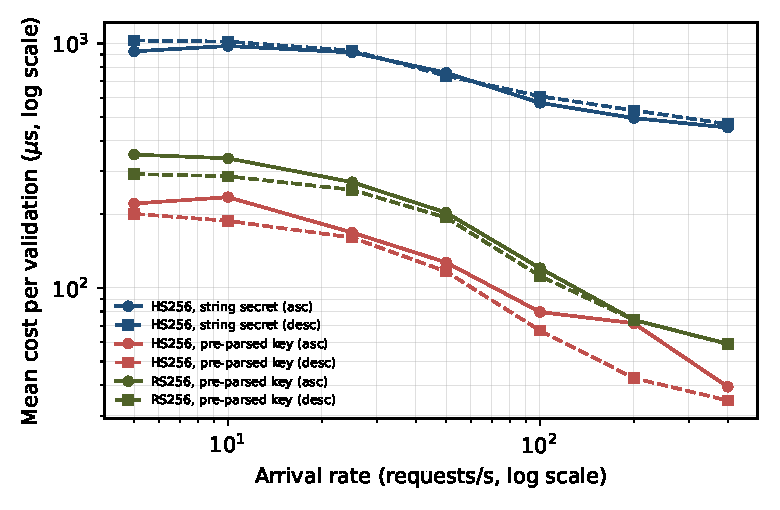
\includegraphics[width=\columnwidth]{fig_insitu_rate.pdf}
\caption{In-situ validation cost against arrival rate, for three key-form and
algorithm combinations, on logarithmic axes. Ascending and descending passes are
drawn separately rather than averaged: Section~\ref{sec:rq3-drift} reports that
they differ systematically, and averaging would conceal that. Every point is
read from a committed run directory by
\texttt{figures/fig\_insitu\_rate.py}~\cite{artifact2026}.}
\label{fig:insitu}
\end{figure}

Two observations follow, both visible in Figure~\ref{fig:insitu}. The cost is
present in deployment and is far larger
than the isolated host figure of Table~\ref{tab:host}, consistent with
Section~\ref{sec:rq2}: the deployed runtime is the one carrying the older
OpenSSL. And the cost depends on arrival rate, falling as the rate rises.

\subsection{The two passes differ systematically}\label{sec:rq3-drift}

Sweeping up and then down is not only replication; it detects warm-up, thermal
and hysteresis effects. If the difference between passes were noise, its sign
would alternate across rate points. It does not. In the string-secret sweep the
descending pass is slower at \InsituStringSameSign{} of \InsituStringPoints{}
rate points; in the pre-parsed sweep the descending pass is \emph{faster} at
\InsituPreparsedSameSign{} of \InsituPreparsedPoints. A consistent sign across
seven points is not what noise produces.

This has a direct consequence for how the ranges in Table~\ref{tab:insitu}
should be read. A systematic component means the two passes are not independent
samples of a common value, so the range between them understates uncertainty
further than a range of two already does. We therefore report ranges and draw no
inference that depends on their width. It is also a methodological finding in
its own right: a single-direction sweep would have produced a curve carrying a
consistent bias with no way to detect it.

\subsection{Host load, not the condition, drives the outliers}\label{sec:rq3-load}

Agreement between passes varies considerably across windows. We distinguish
\emph{relative} disagreement, the gap between passes as a fraction of their
mean, from \emph{absolute} disagreement, the gap in microseconds; the two
behave differently and the distinction carries this subsection.

The widest \emph{relative} disagreement in the dataset and the tightest occur
at the same arrival rate in different sweeps. The wide one is the highest-load
window in its own sweep on the descending pass, though not on the ascending
pass, whose maximum load falls at a different rate. The tight one, at the same
arrival rate in another sweep, sits at a lower load on both passes and its two
passes agree to within \InsituTightestAgreement~$\mu$s. Relative disagreement
therefore does not track the condition under measurement.

We considered two alternative explanations for the relative asymmetry and
reject both. A small-mean effect would require \emph{absolute} disagreement to
be roughly constant, so that its relative size grew only as means shrank;
absolute disagreement instead varies over three orders of magnitude and is
largest where the means are largest, which is the opposite pattern. A
measurement floor would require the affected values to sit at the instrument's
resolution; they do not, and in any case the means reported here are computed
from the histogram's sum and count rather than from its buckets, so bucket
resolution cannot bound them.

The operative consequence is that in-situ figures are reported with the host
load recorded during their window, and comparisons between windows at different
loads are not treated as comparisons between conditions.

\subsection{Corroboration: the cost is real processor time}\label{sec:rq3-ab}

That the in-situ cost is processor time rather than queueing or scheduling
delay is corroborated by an A/B of the same service with validation enabled and
disabled. Table~\ref{tab:ab} gives it here rather than leaving it in the
replication package~\cite{artifact2026}, because the claim it carries is
load-bearing for everything after it.

\begin{table}[t]
\caption{Validation enabled against validation disabled, at one arrival rate.
Two \AbWindowSecondsJwt~s windows on the same pod running the same image
digest, switched by an environment variable, with \AbRequestsNone{} requests in
each. A signed token is on the wire in both arms, so what the disabled arm
removes is the handler's \texttt{jwt.verify()} call and the header reads around
it, not the token. Application and sidecar CPU are means of the one-second
cgroup samples falling inside the window; per-call CPU is that mean divided by
the achieved rate. Event-loop lag is the mean of the per-scrape p99 and is not
a p99 over the window. Host load is the load average sampled at window start;
these two runs carry no within-window load series, so no window mean of it
exists to report.}
\label{tab:ab}
\setlength{\tabcolsep}{4.5pt}
\begin{tabular}{@{}lrr@{}}
\toprule
 & disabled & enabled \\
\midrule
Achieved rate (requests/s)     & \AbRateNone                & \AbRateJwt \\
Application CPU (m)            & \AbCpuNone                 & \AbCpuJwt \\
\textbf{CPU per call ($\mu$s)} & \textbf{\AbCpuPerCallNone} & \textbf{\AbCpuPerCallJwt} \\
Sidecar CPU (m)                & \AbSidecarCpuNone          & \AbSidecarCpuJwt \\
Event-loop lag (ms)            & \AbEventLoopLagNone        & \AbEventLoopLagJwt \\
Client mean (ms)               & \AbLatencyNone             & \AbLatencyJwt \\
Client p99 (ms)                & \AbLatencyPNineNineNone    & \AbLatencyPNineNineJwt \\
Host load, 1 min               & \AbLoadOneNone             & \AbLoadOneJwt \\
Host load, 5 min               & \AbLoadFiveNone            & \AbLoadFiveJwt \\
Host load, 15 min              & \AbLoadFifteenNone         & \AbLoadFifteenJwt \\
\bottomrule
\end{tabular}
\end{table}

Enabling validation adds \AbCpuDelta{} millicores of application CPU at
\AbRateJwt{} requests per second, which is \AbCpuPerCallDelta~$\mu$s of
processor time per call. That is the corroborating figure: it is arrived at
from cgroup CPU accounting, independently of the histogram, and it is the same
order as the in-situ means of Table~\ref{tab:insitu}. Queueing and scheduling
delay are not what moved. Event-loop lag is unchanged between the arms, and the
client-side mean rises by \AbLatencyDeltaUs~$\mu$s, close to the CPU figure
rather than in excess of it, which is what synchronous work on an unsaturated
event loop produces.

The two windows are not at equal host load, and the rule stated above bars us
from comparing them on wall-clock. It does not bar the CPU comparison, which is
what the claim rests on: host contention inflates elapsed time, whereas the
application container's own cgroup accounting measures the processor time it
was charged. Three further observations weigh against reading the CPU
difference as an artefact of the windows. The sidecar, in the same pod under
the same contention, did not rise with it: \AbSidecarCpuNone{} millicores
against \AbSidecarCpuJwt. The per-second samples of the two arms do not
overlap at all --- disabled never exceeded \AbCpuSampleMaxNone{} millicores in
\AbCpuSamplesNone{} samples, enabled never fell below \AbCpuSampleMinJwt{} in
\AbCpuSamplesJwt{} --- which separates the arms without assuming anything about
the distribution, as a test over autocorrelated one-second samples would have
to. And the two host-load indicators disagree in sign: the load average was
higher entering the enabled window, while the busiest process on the host at
that instant was lower there than in the disabled window, \AbTopProcPctJwt\%
against \AbTopProcPctNone\%. The enabled window began \AbGapSeconds~s after the
disabled window ended, and a one-minute load average decays over about that
interval, which is the likeliest reading of a gap that narrows from the
one-minute to the fifteen-minute figure.

What the A/B does not do is attribute the cost within validation. It brackets
the whole \texttt{jwt.verify()} call; Section~\ref{sec:rq1} is what divides it.

\subsection{How common is the avoiding pattern?}\label{sec:rq3-prevalence}

Three instruments, three frames, reported separately as
Section~\ref{sec:method-survey} requires.

\paragraph{Population co-occurrence.} Of \PopJsRequireFiles{} public JavaScript
files importing the library through \texttt{require}, \PopJsRequireFilesWithApi{}
also mention the pre-parsing interface; for JavaScript through \texttt{import}
the figures are \PopJsImportFiles{} and \PopJsImportFilesWithApi; for TypeScript
through \texttt{require}, \PopTsRequireFiles{} and \PopTsRequireFilesWithApi;
and for TypeScript through \texttt{import}, \PopTsImportFiles{} and
\PopTsImportFilesWithApi. Cells are not pooled into a rate: a file using both
import forms would be counted twice, so their sum \PopSumFiles{} is an upper
bound on the union and the largest cell \PopLargestCellFiles{} a lower bound. No
cell exceeds \PopWorstCellPct\% of files mentioning the interface. These are
search-engine estimates of file counts captured on \PopCapturedAt, they cover
public repositories only, and they measure co-occurrence rather than use. The
denominators are returned \emph{rounded} --- each is an exact multiple of
$1024$ --- so they should be read as magnitudes rather than as counts we
established file by file.

\paragraph{Classified call sites.} Of \SampleCallSites{} call sites classified
across \SampleRepos{} distinct repositories, \SampleSitesPreparsed{} pass a
pre-parsed key. Environment variables account for \SampleEnvString{} of those
call sites, untraced identifiers and member expressions \SampleUnknown{}, string
literals \SampleStringLiteral{}, file contents \SampleFileContents{} and buffers
\SampleBuffer. No file in this corpus contains the pre-parsing interface at all,
in any spelling, so the zero reflects the pattern's absence from the sample
rather than a classifier that cannot see it. Incidentally,
\SampleNoAlgorithms{} of \SampleCallSites{} call sites
(\SampleNoAlgorithmsPct\%) pass no algorithm restriction, which
Section~\ref{sec:fix} returns to.

An earlier version of the classifier recognised only the conventional
\texttt{jwt.verify()} spelling, which filtered the corpus toward one import
idiom. It was re-run over the previously unclassified residue with a matcher
that resolves the local binding of the import --- covering arbitrary aliases,
namespace imports, destructured and renamed imports, and direct calls on the
require expression. That recovered \SampleRematchAdded{} further call sites,
included in the totals above, of which \RematchSitesPreparsed{} pass a
pre-parsed key.

\paragraph{Targeted counter-search.} A sample can only show a pattern is rare if
it could have found it. Every file co-occurring the library with the pre-parsing
interface was therefore fetched: \CounterFilesFetched{} files, of which
\CounterWithVerify{} contain a validation call, spanning
\CounterReposWithVerify{} distinct repositories. An automated pass flagged
\AdjudicatedTotal{} call sites as passing a pre-parsed key and all were then
read by hand: \AdjudicatedFalsePositive{} are false positives --- projects
defining their own helper function of the same name, one of which returns a
string --- \AdjudicatedUnresolved{} could not be resolved within its file, and
\AdjudicatedGenuine{} are genuine, across \AdjudicatedGenuineProjects{} distinct
projects.

\paragraph{The rate, with its denominator.} Among the
\CounterReposWithVerify{} repositories that both reference the pre-parsing
interface and call the validator, \AdjudicatedGenuineProjects{} use it: 
\AdjudicatedGenuinePct\%. That denominator is the most favourable available,
since those projects demonstrably know the interface exists, and it is not the
population. The pattern is rare rather than absent, and it is rare even among
projects already aware of it.

\section{A fix, and a constraint on it}\label{sec:fix}

The fix is to dispatch on the token's declared algorithm before attempting the
asymmetric parse, so that an HMAC token with an ordinary string secret is
resolved directly. Applied, this takes the call from \HostJwtString~$\mu$s to
\HostJwtStringSafe~$\mu$s, a factor of \HostSafePatchRatio, and to within
\HostSafePatchResidual~$\mu$s of supplying a pre-parsed key, with no change in
calling code. That residual is the median of the per-round paired differences,
not the difference of the two medians; the two are not identical and the
former is reported throughout.

We tested it against the library's own suite rather than only against
assertions of our own. Cloned at the release tag, the patch applies cleanly and
the suite is unchanged: \SuiteStockPassing{} passing and \SuiteStockFailing{}
failing unpatched, \SuitePatchedPassing{} and \SuitePatchedFailing{} patched.

\paragraph{The constraint, which is the more important half.} The discarded
attempt is not purely wasteful. The \emph{success} of that parse on asymmetric
key material is what produces a key object whose type a later check depends on,
and that check is what prevents symmetric and asymmetric material from being
interchanged~\cite{rfc8725}. A change that dispatches on the declared algorithm
while relaxing which key material may take the fast path alters which inputs
reach that check.

The fix must therefore be narrow: the fast path is restricted to string secrets
that cannot be asymmetric key material, so anything that might be resolves
exactly as it does today. Removing that material restriction --- the form of the
optimisation we argue against --- produces \SuiteNaiveFailing{} failures in the
library's own suite, both in its key-confusion tests.

\paragraph{A reduction of our own contribution.} We had written a regression
test for this property and intended to offer it upstream. Running the library's
existing suite showed that it already constrains the change: a contributor
proposing the unrestricted optimisation would be caught by tests they are
required to run. We therefore withdraw that contribution. What remains is
narrower and, we think, still worth stating: the cost documented in
Section~\ref{sec:rq1} cannot be removed by the obvious route, and the reason is
a property the maintainers already test for but which is not evident from the
code being changed.

The independent defence against this class of confusion is for the caller to
restrict permitted algorithms~\cite{rfc8725}, and
\SampleNoAlgorithmsPct\% of the call sites surveyed in
Section~\ref{sec:rq3-prevalence} do not.

\section{Offloading is not the remedy}\label{sec:offload}

Because a cost believed to be cryptographic invites relocation, we implemented
the relocation the earlier work proposed and report what it does. This section
rests on source inspection and a manual observation; it carries no measured
result, for the reason given below.

\paragraph{The mechanism, which a reader can verify from the source.} Applying a
mesh \texttt{RequestAuthentication} policy causes the sidecar to validate the
token before proxying. It does not cause the application to stop validating:
verification is \emph{duplicated}, not relocated, and no work leaves the event
loop. Making relocation effective therefore requires the application to trust
something the sidecar tells it. In our implementation the handler reads a
sidecar-populated claims header and, when it is present, returns the protected
payload without verifying anything --- the branch is a single conditional in
\texttt{service-a/index.js} in the replication package~\cite{artifact2026}. A
malformed header returns a server error rather than falling back to local
verification, which is the fail-closed behaviour that branch intends.

\paragraph{The observation.} That trust is the vulnerability. The sidecar
overwrites the header only while a policy is applied; in any other state nothing
sanitises it. With the guard filter applied, a request carrying a forged claims
header and no credential at all is refused. With the guard removed, the same
request returns the protected payload. We reproduced this sequence manually ---
refused, served, refused --- and it is consistent with the note recorded
alongside the affected runs in the replication package. The remedy is an
always-applied filter that strips any client-supplied copy of the header on
entry to the pod, before any validation filter runs, matched on the connection
manager rather than on the validation filter, because in the state that needs
protection no validation filter exists.

\paragraph{Why we report no measured result.} We wrote an automated probe to
turn the observation into a table and it does not produce a trustworthy one. The
mesh applies a configuration change asynchronously, on a timescale comparable to
the probe interval, so whether a probe observes the guarded or the unguarded
behaviour depends on whether the proxy had converged when the request fired. Two
runs of the same script produced contradicting values for the same
configuration. Rather than report the run that agreed with our expectation, we
report none: the script's own negative control declared both runs inconclusive,
and we retain it in the replication package with that limitation recorded.
Making this measurable requires gating each probe on \emph{observed}
configuration convergence --- polling until repeated identical responses ---
rather than on a fixed delay. We have not implemented that, and until it is done
this section should be read as a mechanism argument supported by an observation,
not as a measurement.

\section{Implications for practice}\label{sec:implications}

\paragraph{Pre-parse key material once, at startup.} On the host this removes
\HostStringPenalty~$\mu$s per validation
[\HostStringPenaltyCiLo, \HostStringPenaltyCiHi]; on the runtime the service
actually deployed, where the discarded parse costs
\NodeEighteenProbeThrows~$\mu$s, it removes far more. It requires no
architectural change, no new component and no movement of a trust boundary.

\paragraph{Treat the base image as part of the measurement.} The same code, the
same library and the same architecture differ by \SpanProbeThrows$\times$ on
this path across the container images measured, because they pin different
OpenSSL versions. A performance figure quoted without the base image it was
obtained on is not reproducible, and a regression appearing after a base-image
bump may have nothing to do with the application.

\paragraph{Pin the algorithm.} Independently of anything here, callers should
restrict permitted algorithms~\cite{rfc8725}. Most of the call sites we surveyed
do not, which leaves them relying entirely on library-internal key typing for a
property they could assert directly in one argument.

\paragraph{Do not reach for an architectural remedy first.}
Section~\ref{sec:offload} is the argument against treating relocation as the
default response: the cost is not cryptographic, it is largely avoidable in
place, and the remedy that moves validation elsewhere also moves a trust
boundary.

\section{Threats to validity}\label{sec:threats}

\paragraph{One architecture.} Every measurement comes from a single ARM64 host
and its container runtimes under one engine. We have not verified any of this on
x86\_64. The mechanism is a property of a library's API contract --- an
asymmetric parse attempted before a symmetric one, with the failure discarded
--- and of the cost of key parsing in a particular OpenSSL series, and neither
is a property of an instruction set. But an expectation is not a measurement,
and the magnitude in particular depends on how OpenSSL's key parsing performs on
a given platform, which is exactly the kind of quantity that varies with
architecture. No claim here should be read as holding beyond ARM64.

\paragraph{Ranges of two, with a systematic component.} The in-situ dispersion
is the range across an ascending and a descending pass. It is not a confidence
interval, and Section~\ref{sec:rq3-drift} shows the two passes differ
systematically rather than randomly, so they are not independent samples of a
common value and the range understates uncertainty further. No inference in this
paper depends on the width of those ranges.

\paragraph{Sampling frames are not interchangeable.} The three prevalence
instruments of Section~\ref{sec:method-survey} have different units and
different selection mechanisms, and none supports a population proportion. The
co-occurrence counts measure two strings appearing in one file, with a
false-positive rate established at \AdjudicatedFalsePositive{} of
\AdjudicatedTotal{} on hand inspection. The classified sample has unknown
inclusion probabilities, a limitation of repository search noted more generally
by Kalliamvakou et al.~\cite{kalliamvakou2014promises}. The counter-search is
selected on the outcome.

\paragraph{The matcher's coverage.} Call sites are found by resolving the local
binding of the import, which covers aliases, namespace imports, destructured and
renamed imports and direct calls on the require expression. It does not resolve
bindings across files, so a project that constructs a pre-parsed key in one file
and validates in another is invisible to this analysis. This is the strongest
threat to Section~\ref{sec:rq3-prevalence}; within-file tracing found no such
case, which is weak evidence against it.

\paragraph{Host load, and the confound that motivated recording it.} The first
claim withdrawn in Section~\ref{sec:correction} failed because host load moved
unrecorded between runs. Every in-situ window here carries the load average
observed during it, and Section~\ref{sec:rq3-load} shows that window-to-window
agreement tracks that load rather than the condition. Contention inflates a
duration rather than deflating it, so in-situ figures are upper bounds; but
comparisons between windows at different loads are not comparisons between
conditions, and we do not treat them as such.

\paragraph{One host figure cannot be version-attributed.} The host
decomposition of Section~\ref{sec:rq1} predates the per-measurement OpenSSL
field, and the host's OpenSSL has since moved by a patch release, so the
version that produced those figures is known by run timestamp rather than from
the measurement record. Table~\ref{tab:matrix} therefore leaves the host
OpenSSL cell unrecorded rather than filling it with a version captured later.
The container rows, which carry the attribution of Section~\ref{sec:rq2}, each
record their own.

\paragraph{Token caching is not in the comparison.} A service that caches
verified tokens pays this cost once per token rather than once per request. We
did not measure such a configuration, so the per-request figures here do not
describe a caching deployment.

\paragraph{One rater.} The \AdjudicatedTotal{} automatically flagged call sites
were read and classified by the first author, and the authors are not
disinterested: the paper's
claim is stronger the more of them are false positives, and
\AdjudicatedFalsePositive{} were classified that way. There was no second rater
and no inter-rater agreement to report. The per-case verdicts, the evidence for
each and the hashes of the files they were read from are published so the
adjudication can be repeated, which is weaker than having repeated it.

\paragraph{One library at one version.} The mechanism is specific to one
JavaScript implementation at one release. Whether other implementations or other
language ecosystems attempt key resolution in the same order is unmeasured.

\section{Conclusion}\label{sec:conclusion}

The per-request cost of token validation in this library is real, is worth
attending to, and is not cryptographic: the signature primitive is
\HostHmacString~$\mu$s of a \HostJwtString~$\mu$s call. It is not key conversion
either, which costs \HostCreateSecretKey~$\mu$s. It is a parse attempted in the
wrong order, whose failure is constructed and thrown away on every request at
\HostProbeThrows~$\mu$s, \HostProbeShareOfCall\% of the call. Its price is set
by the OpenSSL version a base image happens to pin, varying
\SpanProbeThrows$\times$ across runtimes while the rest of the validation path
varies by \SpanJwtPreparsed$\times$. The pattern that avoids it is rare: among
\CounterReposWithVerify{} repositories that already reference the pre-parsing
interface and call the validator, \AdjudicatedGenuineProjects{} use it.

We withdraw two earlier claims in reaching this: that layered enforcement drives
the service to event-loop saturation, which rested on a curve that moved with
host load; and that the dominant cost is key conversion, which a direct
measurement of the conversion refutes. Both have the same shape, and it is the
shape this paper's methodology is built to avoid: a cost attributed to the
variable under study while a second variable moved alongside it, unrecorded at
the granularity at which it could change. The methodological lesson is not that
one should measure in deployment. It is narrower: record the identity of the
component whose behaviour is being measured, on every measurement, at the
granularity at which it can change.

\section*{Declarations}

\bmhead{Data availability} The data supporting the results of this study are
openly available in the archived replication package~\cite{artifact2026},
deposited on Zenodo under the DOI given in that reference. It contains all
measurements, the instrumentation, the analysis code and the scripts that
generate every numeric value and the figure in this paper. Every number is generated from a
file under the run or survey directories; none is entered by hand. The survey
corpus is third-party source and is not redistributed; a manifest pinning every
file examined by content hash stands in for it, covering \ManifestFiles{} files
across \ManifestRepos{} repositories. Content hashes resolved for all of them;
the repository HEAD commit resolved for \ManifestHeadResolved{} of
\ManifestFiles, one repository having become unavailable between fetch and
manifest. The content hash is the authoritative pin and is complete.

\bmhead{Competing interests} The authors declare no competing interests.

\bmhead{Funding} \textbf{[To be completed by the authors before submission.]}

\bmhead{Author contributions} \textbf{[To be completed by the authors before
submission. Springer requires a statement of each author's contribution; the
present authors' individual roles are not recorded in the artifact and are not
inferable from it.]}

\bmhead{Ethics approval} Not applicable. This study measures software
behaviour and publicly available source code; it involves no human participants
and no personal data.

\bibliography{discarded-exception}

\end{document}
